\documentclass[root.tex]{subfiles}
\begin{document}


\section{Contrôle du bras Jaco dans le simulateur Gazebo par l'entremise de ROS}

Cette section traite d'un environnement de travail hautement versatile permettant la représentation de plusieur architectures de robots.
Pour les besoins du rapport, seulement un exemple avec le bras Jaco sera discuté.
De plus, la complexité de ROS et du simulateur Gazebo oblige de restreindre la présente section à la description sommaire des étapes nécessaires à la mise en marche de l'environnement et à l'utlisation de l'exemple fourni.
Les descriptions fournies ne cherchent pas à être fondamentalement exactes, mais plutôt à expliquer de manière intuitive et succincte le fonctionnement de l'infrastructure à des lecteurs non-initiées.
Il est important de noter que cet environnement est disponible seulement sur les plateforme Linux.

\subsection{Description de l'architecture générale de ROS}

ROS, \textit{robot operating system}, peut être décrit comme un ensemble de programmes (\textit{noeuds}) pouvant fonctionner de manière indépendante, entre lesquels des cannaux de communications standardisés sont établis.
Ces programmes communiquent entre eux en publiant l'information dans une liste des différents sujets (\textit{topics}) publiés par les noeuds présentement en fonctionnement.
Pour obtenir l'information publiée, un autre noeud peut s'abonner au sujet et ainsi lire l'information.

\subsection{Description du simulateur Gazebo}

Gazebo est un simulateur 3D pouvant fonctionner sans nécessiter l'instalation de ROS.
Cependant, il existe une version intégrée de Gazebo dans ROS Kinetic, la version de ROS utilisée pour Ubuntu 16.04.
Gazebo peut être vu comme un noeud ROS qui publie des information par rapport aux différent composants de la simulation.
En utilisant le standard de fichier URDF, c'est dans ce programme que le robot est défini et que les contrôleurs des articulations sont créés.
Suivant la création du robot, Gazebo publie ainsi les informations de l'état du robot et s'abonne à des topics permettant la reception de commandes de moteurs.
La Figure \ref{fig:gazebo_jaco} représente l'interface du simulateur Gazebo lorsque le robot Jaco est configuré.

\begin{figure}
 \begin{center}
  \begin{tabular}{c}
    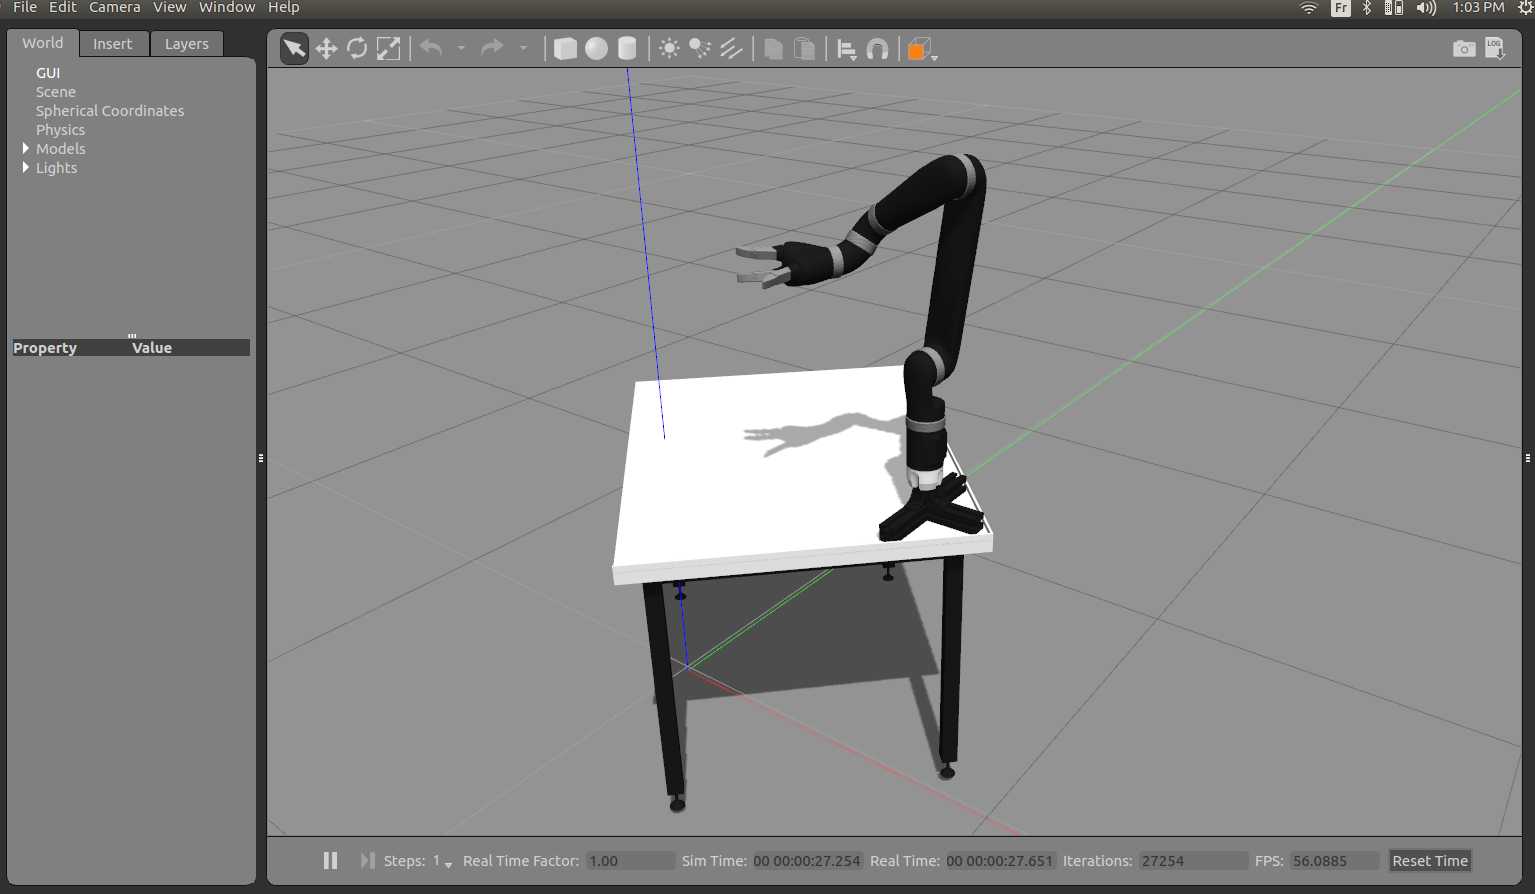
\includegraphics[trim=0cm 0cm 0cm 0cm, scale=0.25]{gazebo_jaco.png}
  \end{tabular}
 \end{center}
\caption{Interface du simulateur Gazebo avec le robot Jaco configuré}
 \label{fig:gazebo_jaco}
\end{figure}

La configuration du robot Jaco à été adaptée d'une suite de programmes (package) open-souce publiée par \cite{jaco_github}.

\subsection{Installation de ROS et de Gazebo}

Comme mentionné plus haut ROS est disponible seulement sur les systèmes d'exploitation Linux.
La séquence d'instructions suivante assume que le système d'exploitation Ubuntu 16.04 est fraichement installé.

\begin{itemize}
\item Aller sur le \href{http://wiki.ros.org/kinetic/Installation/Ubuntu}{site web suivant}.
\item Dans un invité de commande (terminal), entrer, dans l'ordre, les commandes aux étapes 1.2 et 1.3 du tutoriel.
\item Dans un terminal, entrer la commande: \textit{sudo apt-get install ros-kinetic-desktop-full}. Ceci installe ROS et Gazebo.
\item Dans un terminal, entrer, dans l'ordre, les commandes à l'étape 1.5 du tutoriel.
\item Dans un terminal, entrer la commande: echo "source /opt/ros/kinetic/setup.bash" $>>$ $\sim$/.bashrc
\item Entrer ensuite la commande: \textit{source $\sim$/.bashrc}
\item Dans un terminal, entrer la commande: \textit{sudo apt-get install ros-kinetic-catkin}. Ce programme permet la construction d'un environnement de travail avec ROS.
\item Aller sur le \href{http://wiki.ros.org/catkin/Tutorials/create_a_workspace}{site web suivant}.
\item Entrer les commandes mentionnée dans le tutoriel sur cette page.
\item Dans un terminal, entrer la commande: echo "source $\sim$/catkin\_ws/devel/setup.bash" $>>$ $\sim$/.bashrc
\item Entrer ensuite la commande: \textit{source $\sim$/.bashrc}
\end{itemize}

Après l'exécution de ces étape, un environnement de travail pour ROS et Gazebo a été créé dans le fichier \textit{catkin\_ws} situé dans le répertoire \textit{home} de la plateforme Ubuntu.
Les fichiers sur lesquels le projet repose seront placés dans le sous-fichier \textit{src} de l'environnement de travail.

\subsection{Installation de la suite de programmes Jaco}




\newpage
\end{document}














